% !TeX spellcheck = en_GB
\documentclass[a4paper, 12pt]{scrartcl}

\setkomafont{title}{\rmfamily}
\addtokomafont{disposition}{\rmfamily}

\usepackage[english]{babel}
\usepackage[T1]{fontenc}
\usepackage{lmodern}
\usepackage[utf8]{inputenc}

\usepackage{amsmath}
\usepackage{amssymb}
\usepackage{amsfonts}
\usepackage{amsthm}

\usepackage{hyperref}

%\usepackage{icomma}

\usepackage{graphicx}
\usepackage{subcaption}

\usepackage{enumitem}

\usepackage{placeins}

\usepackage[dvipsnames]{xcolor}
\usepackage{mdframed}

\definecolor{light-gray}{gray}{0.975}


\newmdenv[backgroundcolor=light-gray, linecolor=White, leftmargin=-0.25\paperwidth+0.5\linewidth, rightmargin=-0.25\paperwidth+0.5\linewidth, innerleftmargin=0.25\paperwidth-0.5\linewidth, innerrightmargin=0.25\paperwidth-0.5\linewidth]{algorithm}

% leftmargin=-10pt, rightmargin=-10pt]{algorithm}

\usepackage{tablefootnote} 
\makeatletter 
\AfterEndEnvironment{mdframed}{%
	\tfn@tablefootnoteprintout% 
	\gdef\tfn@fnt{0}% 
}

\newcommand{\bfbeta}{\boldsymbol{\beta}}
\newcommand{\bflambda}{\boldsymbol{\lambda}}
\newcommand{\bfmu}{\boldsymbol{\mu}}
\newcommand{\bfalpha}{\boldsymbol{\alpha}}
\newcommand{\bfx}{\mathbf{x}}
\newcommand{\inner}[2]{\left\langle #1, #2 \right\rangle}
\newcommand{\var}{\operatorname{\mathbb{V}ar}}
\newcommand{\ex}{\operatorname{\mathbb{E}}}

%opening
\title{\vspace{0.7cm}{\Large \textbf{TILM3592\\Advanced Statistical Learning}}\\{\LARGE \bfseries Learning Diary}}
\author{{\large NAME}\\
{ MATR.}}
\date{}

\begin{document}
\maketitle


\section{Linear Model Selection and Regularization, Shrinkage}

The objective is to find a good (``best'') model of the form
\begin{equation}\label{eq:fulllinearmodel}
	\mathbf{y}=\beta_0+\beta_1\bfx_1+\ldots+\beta_p\bfx_p.
\end{equation}
One possible solution would be to just use all of the predictors, this would minimize the sum of the squared residuals on the training set but would not necessarily give a model that generalizes as well as a simpler model.
This phenomenon is called overfitting, the model overfits to the training data and performs worse than a simpler model.
Overfitting is often caused by using a model that is too complex.
For example if we have a training set containing $N$ samples of $p$ predictors we could extend the number of predictors until the number of predictors $p'$ is equal to $N$, using some suitable method of extending (for example by constructing suitable polynomials of the initial predictors).
Using all $p'$ of the predictors we would then be able to perfectly fit the training set but performance on the validation set would be awful.

In order to find a model that generalizes well we instead look for a restriction of the model (\ref{eq:fulllinearmodel}) that performs well on a hold out set/test set/validation set.
The restriction can be chosen in many ways, for example we could simply choose the best subset of the predictors.

%\newpage
\subsubsection*{Best Subset Selection}
\begin{algorithm}
For $k=1,\ldots,p$ fit all the ${p \choose k}$ models with $k$ predictors.
For each $k$ choose the model $\mathcal{M}_k$ that performs the best, here the best model can be defined as lowest $R^2$ since all the models have the same number of predictors \tablefootnote{Why not use lowest cross-validation error here too? Perhaps for computational reasons or if no validation set exists.}.
In the end choose the final model by looking at some measure that take into account the complexity of the model (how many predictors were used, $k$) or just using the cross-validation error (either the one predicted using $k$-fold cross-validation or just the performance on a hold-out set).
There are a couple of regularly used measures that take into account the complexity of the model, for example the Akaike and Bayesian Information Criteria, Mallow's $C_p$ or the adjusted $R^2$-statistic.
\end{algorithm}

This method is computationally very expensive if the number of predictors $p$ is large.
This can be seen by looking at the sum of the binomial coefficients, $\sum_{k=0}^{p}{p \choose k}$ which equals $2^p$.
Thus $2^p$ models need to be fit and evaluated before we arrive at a final model.
There are other methods that also perform well (but they might not find the best model) with smaller algorithmic complexity.

\subsection{Stepwise Selection}
Instead of considering all $2^p$ of the models that the best subset selection  algorithm does the following algorithms only consider $p(p+1)/2+1$ models, drastically cutting down on the amount of needed work.
For both of the following algorithms this is done by iteratively starting with some model and modifying it.


\subsubsection*{Forward Stepwise Selection}
\begin{algorithm}
Forward stepwise selection starts with $\mathcal{M}_0$ which is the model containing only the intercept term.
The next model, $\mathcal{M}_1$, is selected by considering the $p$ models we get by including each of the $p$ predictors left separately.
The best of these models is the one with lowest $R^2$ and is denoted with $\mathcal{M}_1$.
This process of selecting one predictor to add to the model at each step is repeated until the model contains all predictors ($p$ times).
The selection fo the final model is similar to the final model selection of the best subset selection algorithm, using some criteria that takes model complexity into account.

At step $k=1,\ldots,p$ we need to fit and evaluate $p-(k-1)$ models.
The total number of models evaluated is then
\begin{equation*}
\sum_{k=1}^{p} \left(p-(k-1)\right) + 1=1+\sum_{k=1}^{p} k = p(p+1)/2+1,
\end{equation*}
where the final $+1$ term is for fitting the $\mathcal{M}_0$ model.
\end{algorithm}

%\begin{mdframed}[backgroundcolor=Goldenrod, linecolor=White]

\subsubsection*{Backwards Stepwise Selection}
\begin{algorithm}
In contrast to forwards stepwise selection backwards stepwise selection is when we start with the full model, $\mathcal{M}_p$, and remove one predictor at each step to iteratively get the models $\mathcal{M}_{p-1},\mathcal{M}_{p-2},\ldots,\mathcal{M}_0$.
The selection of a final model is again the same as for best subset selection and the analysis of complexity is the same as for forwards stepwise selection.
\end{algorithm}

An important thing to note is that stepwise selection does not necessarily give the same model as best subset selection (in other words, not always the best model).
This is because once a predictor is included/dropped we can not choose to drop/reinclude it at a later point even though that might be advantageous.

There are also other ways of doing forwards and backwards stepwise selection, for instance we can choose to use the $F$-statistic to evaluate what predictors to include/drop.

\subsection{Regularization, Shrinkage}
Another approach is to modify the loss-functions used in ordinary linear regression.
Often this is done by adding some kind of penalty to the loss-function, e.g. instead of solving
\begin{equation*}
	\operatornamewithlimits{argmin}_{\bfbeta}\left( \sum_{i=1}^{N}\left(y_i-\beta_0-\bfx_i^\intercal\bfbeta \right)^2\right)
\end{equation*}
we solve
\begin{equation*}
	\operatornamewithlimits{argmin}_{\bfbeta}\left( \sum_{i=1}^{N}\left(y_i-\beta_0-\bfx_i^\intercal\bfbeta\right)^2+\text{penalty}\right)
\end{equation*}
where the penalty often is some function of the coefficients that biases the algorithm towards a simpler model.

\subsubsection*{Ridge Regression}
\begin{algorithm}
Penalize the coefficients by choosing $\lambda\left\|\bfbeta\right\|^2$ as the penalty function.
The optimization problem to be solved is then
\begin{equation*} \hat{\bfbeta}^\mathrm{r}=\operatornamewithlimits{argmin}_{\bfbeta}\left( \sum_{i=1}^{N}\left(y_i-\beta_0-\bfx_i^\intercal\bfbeta\right)^2+\lambda\left\|\bfbeta\right\|^2_2\right),
\end{equation*}
where $\lambda$ is a positive real-valued (tuning) parameter chosen by cross-validation.
The solution is given by
\begin{equation*}
	\hat{\bfbeta}^\mathrm{r}=\left(\mathbf{X}^\intercal\mathbf{X}+\lambda\mathbf{I}\right)^{-1}\mathbf{X}^\intercal\mathbf{y}
\end{equation*}
where $\mathbf{X}$ is the $\left(N\times p\right)$ matrix containing all the observations.
\end{algorithm}

%TODO In practice SVD is useful for solving? PCs?

\subsubsection*{Lasso Regression}
\begin{algorithm}
Instead of penalizing the regular euclidean (2-) norm of the coefficient $\bfbeta$ we penalize the 1-norm of $\bfbeta$.
The optimization problem is then of the form
\begin{equation}\label{eq:lasso}
	\bfbeta^\mathrm{l}=\operatornamewithlimits{argmin}_{\bfbeta}\left(\sum_{i=1}^{N}\left(y_i-\beta_0-\bfx_i^\intercal\bfbeta\right)^2+\lambda\left\|\bfbeta\right\|_1\right)
\end{equation}
with no analytical solution.
Since no analytical solution exists many efficient methods of numerically solving the optimization problem have been developed, many based on techniques in optimization theory and convex analysis.
Here $\lambda$ is also a tuning parameter determined using cross-validation.
\end{algorithm}

Analysing the role of the $\lambda$-parameter a bit more we discover that if we try to use Lagrange multipliers to solve the following optimization problem
\begin{equation*}
	\begin{aligned}
	\operatornamewithlimits{argmin}_{\bfbeta} & & &\left(\sum_{i=1}^{N}\left(y_i-\beta_0-\bfx_i^\intercal\bfbeta\right)^2\right)\\
	\text{subject to} & & & \left\|\bfbeta\right\|_1 \leq t
	\end{aligned}
\end{equation*}
we recover the optimization problem (\ref{eq:lasso}) solved in Lasso regression (up to some constants that do not matter when solving for stationary points of the Lagrange function).
There is then a one-to-one correspondence between the parameters $\lambda$ and $t$ and solving either problem is the same as solving the other problem for some particular combination of parameters.

The interpretation is that the coefficient $\bfbeta$ is constrained to the 1-sphere (a square standing on one corner in 2 dimensions) with radius $t$.
Figure \ref{fig:lassopenalty} illustrates how this can have the effect of selecting variables by choosing $\bfbeta^\mathrm{l}$ such that some coordinates are equal to 0, meaning that some covariates are left outside of the final model.

For ridge regression the same can be done but here the result is that the coefficients are restricted to the regular (Euclidean) 2-sphere (a circle in 2 dimensions).
This does not in general have the effect of selecting variables, which can be seen in figure \ref{fig:ridgepenalty}.

\begin{figure}[h]
	\begin{subfigure}{.5\textwidth}
		\centering
		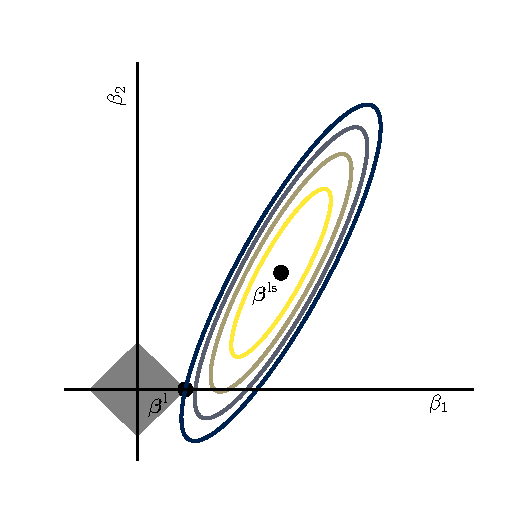
\includegraphics[width=.8\linewidth, clip, trim={10mm 10mm 10mm 10mm}]{Figure1.pdf}
		\label{fig:lassopenalty}
		\caption{Result of Lasso regression with $t=1$.}
	\end{subfigure}
	\begin{subfigure}{.5\textwidth}
		\centering
		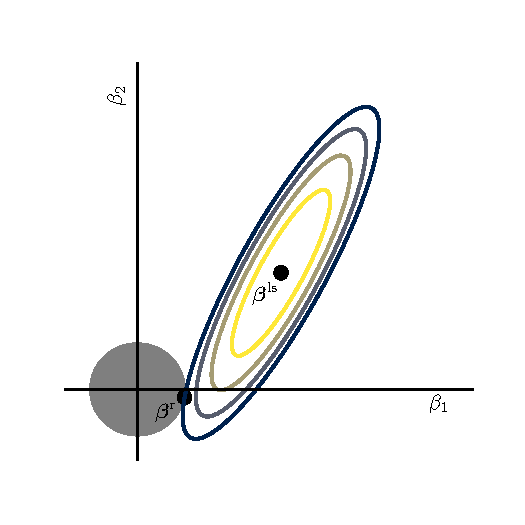
\includegraphics[width=.8\linewidth, clip, trim={10mm 10mm 10mm 10mm}]{Figure2.pdf}
		\label{fig:ridgepenalty}
		\caption{Result of ridge regression with $t=1$.}
	\end{subfigure}
	\caption{Figures illustrating the effect of the variables $t$ and $\lambda$ on the optimal values.
	The coefficient chosen by ordinary least squares is indicated by $\bfbeta^\mathrm{ls}$ with Lasso and ridge regression coefficients indicated by $\bfbeta^\mathrm{l}$ and $\bfbeta^\mathrm{r}$.
	The contours are the error (lines) and penalty (grey) parts of the loss function.}
\label{fig:fig}
\end{figure}


\subsection{Linear models utilising dimensionality reduction}
First we acquaint ourselves with a common method for dimensionality reduction.
The idea when doing dimensionality reduction is to represent the data in a less complex way without losing too much information.
For example we can try to represent the data in a new coordinate system with a smaller dimension than before while keeping as much of the variance in the model as possible.

\subsubsection*{Principal Components Analysis}
Principal components analysis is when the idea above is implemented so that we first try to find a vector $\mathbf{v}_1$ to project the new data on such that the variance of the projection is maximized.
The variance of a random variable is defined as $\var\left(\bfx\right):=\ex\left[\left(\bfx-\bfmu\right)^\intercal\left(\bfx-\bfmu\right)\right]=\ex\left(\inner{\bfx-\bfmu}{\bfx-\bfmu}\right)$ and if the random variable is centred so that the mean is equal to $\mathbf{0}$ this is equal to just $\ex\left(\bfx^\intercal\bfx\right)=\ex\left(\inner{\bfx}{\bfx}\right)$.
The projection of a random variable $\bfx$ on a vector $\mathbf{v}$ is equal to $\frac{\inner{\bfx}{\mathbf{v}}\mathbf{v}}{\left\|\mathbf{v}\right\|^2}$ where the scalar $\frac{\inner{\bfx}{\mathbf{v}}}{\left\|\mathbf{v}\right\|}$ says how far along the unit vector $\frac{\mathbf{v}}{\left\|\mathbf{v}\right\|}$ we should travel so that the random variable $\bfx$ is as close as possible.
Since all the projections will be lying on the vector $\mathbf{v}$ it is enough to take the difference between the scalars $\frac{\inner{\bfx}{\mathbf{v}}}{\left\|\mathbf{v}\right\|}$ when calculating the variance.
The variance of the projection is then equal to:
\begin{equation*}
	\var\left(\frac{\inner{\bfx}{\mathbf{v}}}{\left\|\mathbf{v}\right\|}\right)=\ex\left[\left(\frac{\inner{\bfx}{\mathbf{v}}}{\left\|\mathbf{v}\right\|}\right)^\intercal\left(\frac{\inner{\bfx}{\mathbf{v}}}{\left\|\mathbf{v}\right\|}\right)\right]=\ex\left[\frac{\left(\bfx^\intercal\mathbf{v}\right)^\intercal\left(\bfx^\intercal\mathbf{v}\right)}{\left\|\mathbf{v}\right\|^2}\right]=\ex\left[\frac{\mathbf{v}^\intercal\bfx\bfx^\intercal\mathbf{v}}{\mathbf{v}^\intercal\mathbf{v}}\right].
\end{equation*}
Using $N$ samples $\bfx_1,\dots,\bfx_N$ this can be estimated by summing over the result of the previous calculation for each sample and dividing by the number of samples but since the number of samples is fixed we can ignore this step.
This can also be expressed in matrix notation by stacking the samples $\bfx_i$ as rows in $\mathbf{X}$.
The sum is then represented by the quantity
\begin{equation*}
	\frac{\mathbf{v}^\intercal\mathbf{X}^\intercal\mathbf{X}\mathbf{v}}{\mathbf{v}^\intercal\mathbf{v}}.
\end{equation*}

Finding a vector $\mathbf{v}$ that maximizes the variance of a random variable $\bfx$ projected upon it is then equal to solving the following optimization problem:
\begin{equation*}
\begin{aligned}
	\operatornamewithlimits{argmax}_{\mathbf{v}_1} & & &\frac{\mathbf{v}_1^\intercal\mathbf{X}^\intercal\mathbf{X}\mathbf{v}_1}{\mathbf{v}_1^\intercal\mathbf{v}_1}.
\end{aligned}
\end{equation*}
Scaling the vector $\mathbf{v}$ does not change the value of the objective function here so we can add the constraint $\left\|\mathbf{v}\right\|=1$ to get a unique solution. The optimization problem is then
\begin{equation*}
\begin{aligned}
\operatornamewithlimits{argmax}_{\mathbf{v}_1} & & &\mathbf{v}_1^\intercal\mathbf{X}^\intercal\mathbf{X}\mathbf{v}_1\\
\text{subject to} & & &\left\|\mathbf{v}\right\|=1
\end{aligned}
\end{equation*}
with the Lagrange function
	$\mathcal{L}\left(\mathbf{v}_1, \lambda_1\right)=\mathbf{v}_1^\intercal\mathbf{X}^\intercal\mathbf{X}\mathbf{v}_1-\lambda_1\left(\mathbf{v}_1^\intercal\mathbf{v}_1-1\right)$.
Stationary points are found by solving for points where the derivative $\frac{\mathrm{d}\mathcal{L}}{\mathrm{d}\mathbf{v}_1}=2\mathbf{v}_1^\intercal\mathbf{X}^\intercal\mathbf{X}-2\lambda_1\mathbf{v}_1^\intercal$ equals 0.
This is obviously an eigenvalue problem and the solution is given by the largest eigenvalue $\lambda_1$ of the matrix $\mathbf{X}^\intercal\mathbf{X}$  with the corresponding eigenvector $\mathbf{v}_1$.

The first \emph{principal component} of an observation $\bfx_i$ is what the projection $\inner{\bfx_i}{\mathbf{v}_1}\mathbf{v}_1$ is called.
In order to find more principal components the data can be altered by subtracting the projections of the samples on the eigenvectors and then extracting a new eigenvector in a similar way.
It turns out that first eigenvector of the new (squared) data matrix will be the second eigenvector of the original and this is starting to look a lot like some sort of eigenvector decomposition of the matrix $\mathbf{X}^\intercal\mathbf{X}$ or $\mathbf{X}$, which is the approach investigated below. 

The other approach is to model the observations as the rank-$q$ linear model $f(\bflambda)=\bfmu + \mathbf{V}_q\bflambda$ where $\bflambda$ are coordinates in a $q$-dimensional space, $\bfmu$ is the location of the $p$-dimensional mean and $\mathbf{V}_q$ is a $\left(q\times p\right)$-dimensional matrix with $q$ orthonormal vectors as columns.
This is an affine hyperplane of rank $q$.
\begin{algorithm}
	We try to minimize the \emph{reconstruction error}:
	\begin{equation*}
	\begin{aligned}
		\operatornamewithlimits{argmin}_{\bfmu, \bflambda_i, \mathbf{V}_q} & & &\sum_{i=1}^{N}\left\|\bfx_i-\bfmu-\mathbf{V}_q\bflambda_i\right\|^2.
	\end{aligned}
	\end{equation*}
	By partially optimizing for $\boldsymbol{\mu}$ and $\bflambda_i$ we get $\hat{\boldsymbol{\mu}} = \bar{\bfx}$ and $\hat{\bflambda}_i=\mathbf{V}_q^\intercal \left(\bfx_i-\bar{\bfx}\right)$.
	Assuming the data is centred ($\bar{\bfx}=\mathbf{0}$) we are left with determining $\mathbf{V}_q$:
	\begin{equation*}
	\begin{aligned}
	\operatornamewithlimits{argmin}_{\mathbf{V}_q} & & &\sum_{i=1}^{N}\left\|\bfx_i-\mathbf{V}_q\mathbf{V}_q^\intercal\bfx_i\right\|^2.
	\end{aligned}
	\end{equation*}
	The solution can be constructed using the singular value decomposition $\mathbf{U}\mathbf{D}\mathbf{V}^\intercal$ of the data $\mathbf{X}$.
	Here $\mathbf{U}$ is a $\left(N\times p\right)$ orthogonal matrix, $\mathbf{D}$ is a $\left(p\times p\right)$ diagonal matrix with the eigenvalues of $\mathbf{X}$ on the diagonal ordered by size and $\mathbf{V}^\intercal$ is a $\left(p\times p\right)$ orthogonal matrix. The solution $\mathbf{V}_q$ for a given $q\leq p$ is given by the first $q$ columns of $\mathbf{V}$.
	Similarly the new reduced space is given by the first $q$ columns of $\mathbf{U}\mathbf{D}$.
	
	The interpretation is that we have projected the original space down on the first $q$ \emph{principal components} of the data.
	We also have a way to reconstruct the original data using the matrix $\mathbf{V}_q$.
\end{algorithm}

Principal components analysis also has a couple of other interpretations and properties.
For example the eigenvalues can be interpreted as the variance explained by a particular principal component.
The total variance is then given by the sum of all the eigenvalues and the ratio of variance explained to total variance is the ratio of the sum of the $q$ largest eigenvalues to the sum of all the eigenvalues.
Normally the decomposition is constructed for all $p$ principal components and a plot of the ratio of variance explained to total variance for each $q$ is used to determine when to stop.
Usually there is a sharp drop of in additional explaining power after a couple of principal components, at that point it is no longer efficient (in the interest of interpretability) to include more dimensions.

\subsubsection*{Principal Components Regression}
Now that we have a method for reducing the dimensionality of our data we could try ordinary linear regression on the new dimensions.
\begin{algorithm}
	Principal components regression is when ordinary linear regression is ran on the first $k$ principal components calculated using PCA.
	The principal components $\mathbf{z}_i$ are given by $\mathbf{z}_i=\mathbf{X}\mathbf{v}_i$ where $\mathbf{v}_i$ are the eigenvectors identified by PCA.
	Stacking the principal components columnwise in an $\left(N\times k\right)$ matrix $\mathbf{Z}$ means that the ordinary least squares solution $\bfalpha^\mathrm{ls}$ to the optimization problem
	\begin{equation*}
	\begin{aligned}
	\operatornamewithlimits{argmin}_{\bfalpha} & & &\left\|\mathbf{y}-\mathbf{Z}\bfalpha\right\|^2.
	\end{aligned}
	\end{equation*}
	is given by $\bfalpha^\mathrm{ls}=\left(\mathbf{Z}^\intercal\mathbf{Z}\right)^{-1}\mathbf{Z}^\intercal\mathbf{y}$, here everything is assumed to be centred (also $\mathbf{y}$).
\end{algorithm}


Using the singular value decomposition we can also compare the least squares and ridge regression solutions.
For least squares we get:
\begin{align*}
	\mathbf{X}\bfbeta^\mathrm{ls}&=\mathbf{X}\left(\mathbf{X}^\intercal\mathbf{X}\right)^{-1}\mathbf{X}^\intercal\mathbf{y}
	=\mathbf{U}\mathbf{D}\mathbf{V}^\intercal\left(\mathbf{V}\mathbf{D}^\intercal\mathbf{U}^\intercal\mathbf{U}\mathbf{D}\mathbf{V}^\intercal\right)^{-1}\mathbf{V}\mathbf{D}^\intercal\mathbf{U}^\intercal\mathbf{y}\\
	&=\mathbf{U}\mathbf{D}\mathbf{V}^\intercal\left(\mathbf{V}^\intercal\right)^{-1}\mathbf{D}^{-2}\mathbf{V}^{-1}\mathbf{V}\mathbf{D}\mathbf{U}^\intercal\mathbf{y}
	=\mathbf{U}\mathbf{U}^\intercal\mathbf{y},
\end{align*}
while for ridge regression the result is
\begin{align*}
	\mathbf{X}\bfbeta^\mathrm{r}&=\mathbf{X}\left(\mathbf{X}^\intercal\mathbf{X}+\lambda\mathbf{I}\right)^{-1}\mathbf{X}^\intercal\mathbf{y}
	=\mathbf{U}\mathbf{D}\mathbf{V}^\intercal\left(\mathbf{V}\mathbf{D}^\intercal\mathbf{U}^\intercal\mathbf{U}\mathbf{D}\mathbf{V}^\intercal+\lambda\mathbf{I}\right)^{-1}\mathbf{V}\mathbf{D}^\intercal\mathbf{U}^\intercal\mathbf{y}\\
	&=\mathbf{U}\mathbf{D}\mathbf{V}^\intercal\left(\mathbf{V}\mathbf{D}\mathbf{D}\mathbf{V}^\intercal+\lambda\mathbf{I}\right)^{-1}\mathbf{V}\mathbf{D}^\intercal\mathbf{U}^\intercal\mathbf{y}
	=\mathbf{U}\mathbf{D}\mathbf{V}^\intercal\left(\mathbf{V}\mathbf{D}\mathbf{D}\mathbf{V}^\intercal+\lambda\mathbf{V}^\intercal\mathbf{V}\right)^{-1}\mathbf{V}\mathbf{D}^\intercal\mathbf{U}^\intercal\mathbf{y}\\
	&=\mathbf{U}\mathbf{D}\mathbf{V}^\intercal\left(\mathbf{V}\mathbf{D}\mathbf{D}\mathbf{V}^\intercal+\lambda\mathbf{V}^\intercal\mathbf{V}\right)^{-1}\mathbf{V}\mathbf{D}^\intercal\mathbf{U}^\intercal\mathbf{y}
\end{align*}


\end{document}
